\documentclass[]{UCD_CS_FYP_Report}
\usepackage{graphicx}
\usepackage{listings}
\usepackage{hyperref}
\usepackage{amsmath, amssymb, amsthm}
\hypersetup{
    colorlinks=true,
    linkcolor=blue,
    filecolor=magenta,      
    urlcolor=cyan,
}
\lstset{
    mathescape=true,
    basicstyle = \ttfamily
}
%\usepackage[backend=biber,style=chicago-authordate]{biblatex}
\usepackage[backend=biber,style=nature]{biblatex}
\addbibresource{references.bib}


%%%%%%%%%%%%%%%%%%%%%%
%%% Input project details

\def\studentname{Sabeer Bakir}% Edit with your name
\def\studentid{16333886}% Edit with your student id
\def\projecttitle{Learning shortest path tours to all pubs in UK} % Edit with you project title
\def\supervisorname{Deepak Ajwani}


\begin{document}
\maketitle

%%%%%%%%%%%%%%%%%%%%%%
%%% Table of Content

\tableofcontents
%\pdfbookmark[0]{Table of Contents}{toc}\newpage
%\newpage


%%%%%%%%%%%%%%%%%%%%%%
%%% Your Abstract here
\abstract
Designing algorithms for NP-hard combinatorial optimization problems is a complex task. These problems are typically solved using carefully designed heuristics and polynomial time approximation algorithms. However, these solutions require problem-specific knowledge and trial-and-error. Automating this process has been a long-held dream of AI researchers. In this thesis, we consider the Travelling Salesman Problem (TSP) and use a classification model to identify the edges that are contained in the TSP tour. 


%%%%%%%%
\chapter{Project Specification}
\LARGE Core
\normalsize
\begin{itemize}
    \item Identify features of edges that can discriminate between edges in the shortest TSP tour and edges that are not.
    \item Take random samples of the pub crawl dataset and use a state-of-the-art heuristic on that to get the ground truth for training
    \item Use the identified features and the ground truth on random samples to train a classification model that learns the edges in the shortest TSP tour
    \item Evaluate the accuracy of the classification model
\end{itemize}
\LARGE Advanced
\normalsize
\begin{itemize}
    \item Compare the running time vs. optimality trade-off of the learning approach with the Concorde TSP solver (\url{http://www.math.uwaterloo.ca/tsp/concorde.html})
    \item Improve the accuracy of the classification algorithm by careful feature selection
\end{itemize}


%%%%%%%%
\chapter{Introduction}
The Travelling salesman problem (TSP) is a combinatorial graph optimization question that is. This problem is NP-hard and has caused considerable interest by theory and algorithm design communities in the past. In the realm of computational complexity, one of Karp's 21 NP-complete problems is the Hamiltonian Cycle Problem, this is a special case of the travelling salesman problem.\\[0.2cm] 
The TSP was first introduced in the 1800s by the Irish mathematician Sir William Rowan Hamilton and the British mathematician Thomas Penyngton Kirkman. However, optimisation of the TSP only came about in the 1930s from Karl Menger in Vienna and Harvard. Menger defined the problem as, “Given a finite number of points, with known pairwise distances, find the shortest path connecting the points.”\cite{Menger}

Techniques that are used to solve these graph optimisation problems comes in three main type: exact algorithms, approximation algorithms and heuristics. Exact algorithms always find the most optimal solution however it requires exponential time which does not scale well for large inputs. Approximation algorithms offer the desirable polynomial time solution however it is hard to guarantee the optimality for certain problems. Heuristics are typically fast but require problem specific research and experimenting from the algorithm designers.\\[0.2cm]
Designing algorithms for NP-hard combinatorial optimization problems is a complex task. It has been shown with use of good heuristics and approximation algorithms that these problems can be solved in polynomial time. However, these solutions require problem-specific knowledge and trial-and-error. Is it possible to automate this learning process with the use of machine learning classification? In real world applications, the data is very rarely similar however the structures within the data do not differ. In this paper, we will explore a method to solve the Travelling Salesman Problem (TSP) using classification to identify edges that are contained within the tour created by the TSP. We will see if it is possible to learn the shortest path to all pubs in the UK. The applications of this can be applied in many areas such as, DNA Sequencing, Route Planning, Logistics Management, etc.

%%%%%%%%
\chapter{Related Work and Ideas}
\subsection{Background to Combinatorial Optimization}
Combinatorial optimization is an area of research that consists of finding an optimal ordering/subset from a finite set of objects. In many of these problems, exhaustive search is not an option as these problems are NP-hard, meaning that there is no known polynomial time algorithm to solve them. There is a demand for solutions to these problems in many domains such as network design, bioinformatics, game theory and many more \cite{combApplications}. Is it possible to still find good solutions to these problems? Due to the popularity of these problems, it has created a surge of algorithms that approximate a solution close to the optimal solution. These methods include exact algorithms \cite{Bellman:1962:DPT:321105.321111}, approximation algorithms \cite{JohnMcGe97}, domain specific heuristics\cite{davidapplegate2007} and meta-heuristics \cite{Larranaga1999, NatureBasedHeuristics}. The travelling salesman problem is no exception to these methods, the TSP is known as a classic problem in combinatorial optimisation. 

Initially the travelling salesman problem was tackled using exact algorithms, searching for a complete solution. One of the first algorithms of this nature was the Held-Karp Algorithm \cite{Bellman:1962:DPT:321105.321111}. These exact algorithms that searched the entire solution space often were only useful for very small input sizes and was usually not suitable for real world data more nodes and edges than synthetic problems.

\textbf{Exact Algorithms}
An exact algorithm in the domain of optimization refers to a method that will always yield the most optimal solution. Such algorithms do exist for the TSP \cite{Bellman:1962:DPT:321105.321111}, this is one of the earliest adoptions of \textit{Dynamic Programming}. The main disadvantage to this algorithm is its runtime of $\mathcal{O}(N^22^N)$. Due to this, algorithm designers have looked towards other methods of optimisation such as heuristics and approximation algorithms.

\subsection{Approximation Algorithms}
Algorithm designers looked towards approximating the solution such that a close to optimal solution could be obtained in substantially less time than an exact algorithm. Many approximation algorithms have been applied to the travelling salesman problem; one noteworthy method is Christofides \cite{JohnMcGe97}. There has been little to no improvement in approximation algorithms since. 

\textbf{Christofides} ensures solutions that will be within a factor of 3/2 of the optimal solution. The tour is generated by constructing the minimum weight spanning tree where the weights are the distances between the nodes. Compute a perfect matching on the nodes of odd degree and combine with the spanning tree. This will result in a connected graph with each node having even degree. On one hand, this approach has the best worst-case solution of the constructive heuristics, on the other hand it's runtime is substantially longer than heuristics due to the perfect matching algorithm complexity.

\subsection{Heuristics}
Designers looked towards domain specific heuristics to solve TSPs with some prior knowledge of the problem at hand. These methods are fast and will run in polynomial time whilst yielding solutions very close to optimal. An example of such heuristics can be found in the Concorde TSP Solver \cite{davidapplegate2007}, a very powerful program used to solve TSPs with close to optimal solutions on graphs with tens of thousands of nodes.

\textbf{Constructive Heuristics}
This approach differs from local search heuristics where a solution is given and optimality is obtained by making local changes at various points in the solution. Constructive heuristics begin with an empty solution and attempt local optimizations at each point in the solution. In \cite{JohnMcGe97}, algorithms such as \textit{Nearest Neighbour (NN)}, \textit{Greedy}, \textit{Clarke-Wright}, and
\textit{Christofides} are applied to the TSP. 
\begin{itemize}
  \item \textbf{Nearest Neighbour (NN): }This algorithm constructs a tour from starting at some arbitrary node and builds the cycle by adding the nearest neighbour from the current node. It's runtime is $\mathcal{O}(N^2)$. This provides a decent approximation for the most optimal, on average the path length is roughly 25\% longer than the most optimal path.
  \item \textbf{Greedy: }Often mistaken for Nearest Neighbour, it is constructed by taking the complete graph of the TSP instance, and the path starts with the shortest edge. It is further built by continuously adding the next shortest incident edge such that no node has degree greater than 2 or cycle length less than the total number of nodes. Its runtime is slightly longer than that of NN at $\mathcal{O}(N^2logN)$ however the worst case solution is better than NN.
  \item \textbf{Clarke-Wright (CW): }This algorithm originally comes from a vehicle routing method designed by Clarke and Write\cite{Clarke:1964:SVC:2769344.2769349}. In terms of the TSP, an arbitrary city is chosen as a central point for which the salesman would return to after each visit to another city. A \textit{savings} metric is defined as how much shorter the tour becomes if the salesman skips returning to the central point. A greedy approach is then utilized on these savings values rather than the edge distances. Since this is a different approach of the greedy algorithm, it's runtime is similarly $\mathcal{O}(N^2logN)$. This method has a higher best performance in comparison to the greedy algorithm however it's worse case performance is the same.
\end{itemize}

\textbf{Concorde TSP Solver}
In the 1990s, a collection of heuristics and functions have been designed by Applegate, Bixby, Chvátal, and Cook \cite{davidapplegate2007}. This solver holds the most records for solving large TSP instances with minuscule loss in accuracy. This precision does come at the cost of time, many large TSP problems take over 100-years of CPU time which isn't ideal for applications that require solutions to be obtained swiftly. The applications of the Concorde include: gene-mapping\cite{10.1093/jhered/esg012}, protein function prediction\cite{Johnson2006}, vehicle routing\cite{ApplegateVPR}, etc. According to \cite{MULDER2003827}, the Concorde “is widely regarded as the fastest TSP solver, for large instances, currently in existence.”

\newpage
\subsection{Meta-heuristics}
The time taken to develop heuristics can be heavily time consuming. To remedy this learning process, meta-heuristics were implemented to augment algorithm designer’s ability to distinguish the details within the problem instances. Despite this benefit of meta-heuristics, it shifts the problem to properly configuring the algorithm with the correct parameters which can vary from problem to problem. The overall goal of these algorithms is to find a global optimum within the solution space. This is different to regular heuristics that often get trapped in local optimum solutions. Some examples of these methods include: Genetic algorithms, Bee Colony Optimization, Ant Colony Optimization and Particle Swarm Optimization. These solutions introduce a new problem of interpretability of the method, many of these algorithms are considered “black boxes”. It’s very difficult to analyse exactly what is happening, because of this there is no guarantee of an approximation factor.

\textbf{Genetic algorithms}
There have been many different attempts at solving the travelling salesman problem with genetic algorithms. These methods rely heavily on mutation and crossover operators, these operators are trivial for some problems however for the TSP, a representation of the tour should be defined such that these operators can be developed. Most genetic algorithms designed for the TSP are using path representation where the cities are put into an ordered list where the first city in the list is the first city to be visited \cite{Larranaga1999}. Mutation is used to allow the algorithm to explore the solution space to avoid a local optimal solution whereas the crossover operator is used to increase the quality of solutions. This type of method lends itself well to certain problem domains however it does not generalize well to other problems.

\textbf{Nature Based Heuristics}
These types of heuristics apply concepts from nature to tackle complex computational problems. Examples of these heuristics include: Simulated Annealing, Evolutionary Algorithms, Ant Colony Optimization and Particle Swarm Optimization. Each of these methods share an underlying concept in nature and lend itself well to solving optimization problems. In a comparative study of nature inspired heuristics on the travelling salesman problem \cite{NatureBasedHeuristics}, it was found that an iterative local search (ILS) performed the best on most instances. It was surprising to find an ILS algorithm to perform well on a TSP problem, typically these types of methods tend to fall into a local optimum, yielding worse solutions.



\subsection{Deep Learning}
Deep neural networks are powerful frameworks that can take large amounts of data and process it through a series of layers to extract features from the input and produce an output according to what it’s trained to learn. In the case of the travelling salesman problem, the input is the elements of the problem instance, the nodes and edges in graphs. It’s expected output is edges in the travelling salesman problem that are part of the shortest tour. These neural networks automatically learn features relevant to the problem as well as the mapping from the input to the output. However, this mapping is only valid for an instance from a given domain. One of the issues with training a deep neural network is the large amount of training data required to have an accurate model. To acquire such training data, that would involve solving NP-hard problems itself. The way to combat this is to train the network on small instances that are relatively easier to collect training data for as patterns observed in smaller instances remain true for larger instances. \cite{NIPS2015_5866} used a pointer networks to solve the travelling salesman problem, they trained on smaller instances containing 5-20 points. They observed almost perfect results for 25 points, good results for 30 points and the accuracy decreased dramatically for 40 and above. The more glaring issue with deep learning is the interpretability of the method, with large amounts of weights and biases, it becomes very difficult to analyse the solution. The method is not flexible either, adding new constraints or a change to the domain can have dramatic effects on the solution.

\textbf{Deep reinforcement learning}
The use of an \textit{on-policy} techniques using neural networks was applied in \cite{DeepRL} in a framework called \textsc{GCOMB}. Here they explore graph embedding techniques using \textit{Graph Convolutional Networks (GCN)} which are then fed into a neural network to learn a \textit{Q}-function in order to predict a solution. This solution would come in the form of an unordered or ordered set of nodes, depending on the problem. The advantages of this implementation include: 
\begin{itemize}
  \item \textbf{Scalability: }The proposed framework in the above study is able to scale to networks with millions of nodes and billions of edges.
  \item \textbf{Generalizability: }\textsc{GCOMB}'s framework allows itself to be applied to many combinatorial problems rather than focusing on one specific problem.
\end{itemize}
However these advantages do come with the trade-off of interpretability, it becomes difficult to narrow down how the solution came to be with such complex frameworks. We will attempt to remedy this issue in this paper with our proposed framework.

\subsection{Machine Learning}
The machine learning space of combinatorial optimization is currently dominated by reinforcement learning methods and frameworks. Reinforcement learning differs from supervised learning by not requiring input-output pairs of examples to train on. Instead, the algorithm aims to strike a balance between exploration of the solution space and exploiting previously learning knowledge about the solution space \cite{ReinforcementLearning}.

\textbf{Reinforcement learning}
Reinforcement learning is used as a natural framework for learning the evaluation function in \cite{DBLP:journals/corr/DaiKZDS17}. An \textit{off-policy} reinforcement learning algorithm such as \textit{Q}-Learning was utilized here which updates its rules on the Q-Value rather than looking at past examples to learn. This technique was used over graph problems such as: Minimum Vertex Cut (MVC), Maximum Cut (MAXCUT), and the Travelling Salesman Problem (TSP). This type of approach lends itself to designing greedy heuristics for difficult combinatorial optimization problems. Heuristics as we know are commonly fast but in the area of optimization require certain knowledge about the underlying problem, this approach attempts to build these heuristics whilst learning about the underlying problem.

\textbf{Supervised Machine Learning}
There has been recent work in supervised machine learning in \cite{iAAA}. They have built a framework for reducing the search space of the problem by augmenting state-of-the-art solvers to solve the maximum clique problem. This is done by identifying the vertices that are not part of the solution and pruning them from the data such that search space is reduced significantly and an approximation algorithm can be used to find the maximum clique in a shorter time than if this algorithm was run on the full set of vertices.

Our proposed framework will borrow techniques from \cite{iAAA} and apply it to the travelling salesman problem.




%%%%%%%%
\chapter{Data Considerations}
The data is comprised of locations of pubs within the UK scraped from \url{https://www.pubsgalore.co.uk/}, a site containing addresses of all the pubs within the UK. The gathered data will include the name of each pub, a longitude and latitude pair, and if the pub is open or closed.  Upon inspection there is roughly 70000+ pubs. The data will be static and locally stored. We are using this as our primary source of data as it is regularly kept up to date and has very few missing values.

There is plenty of cleaning and pre-processing to be completed on the data. Converting the points to an edge list of a complete graph such that each point has an edge to every other point, calculating the weights of each edge (Euclidian distance between points), creating features for the edges and generating the ground truth for each edge.

We will be using the Concorde TSP Solver \cite{davidapplegate2007} to build a tour from our dataset. This will provide us with the edges that are in the solution set and will help create our target for each instance in the original data.
All the data used in this paper will be made publicly available. Any data used in this project was fairly gathered and raises no ethical concerns.


%%%%%%%%
\chapter{Outline of Approach}
\subsection{Problem Statement}
In our case, lets assume for an instance of the travelling salesman problem, it is represented as an undirected weighted graph $G = (V, E, w), w:E\to\mathbb{R}$, where each weight corresponds to the distance from each point. $V$ is the set of cities/points in the graph and $E$ is the edges/arcs that connect them. For each problem instance, let $G$ be a complete graph such that every pair of distinct vertices is joined by an edge.

The goal is to create a tour that traverses this graph, crossing every vertex in $V$ with minimal weight and return to beginning of the tour. Such a tour is known as a \textit{Hamiltonian cycle}.

\subsection{Approach}
We will attempt to use a simple binary classification model to learn whether an edge is part of the TSP tour or not. The advantage to this approach is the interpretability and scalability of this model over more complex frameworks such has deep learning. We will be able to analyse the parameters and see the key features that distinguish edges from each other.

We will be training several classifiers such as:
\begin{itemize}
    \item Random Forest: Each tree within the forest will be trained on different types of graph structures (i.e. big cities, islands, rural areas, etc.). Majority voting from these trees will make calculate whether an edge is contained within the tour. 
    \item Naïve Bayes
    \item Linear Regression
\end{itemize}

The other classifiers will be used to compare the performance of the Random Forest algorithm.
Start with small subsets of the data (i.e. 1000 points), as the algorithm improves, we will increase the input size until we are able to fully classify the entire dataset.
We will prune\cite{iAAA} the edges that are guaranteed not to be contained within the tour. 

\newpage
\begin{figure}[h]
    \centering
  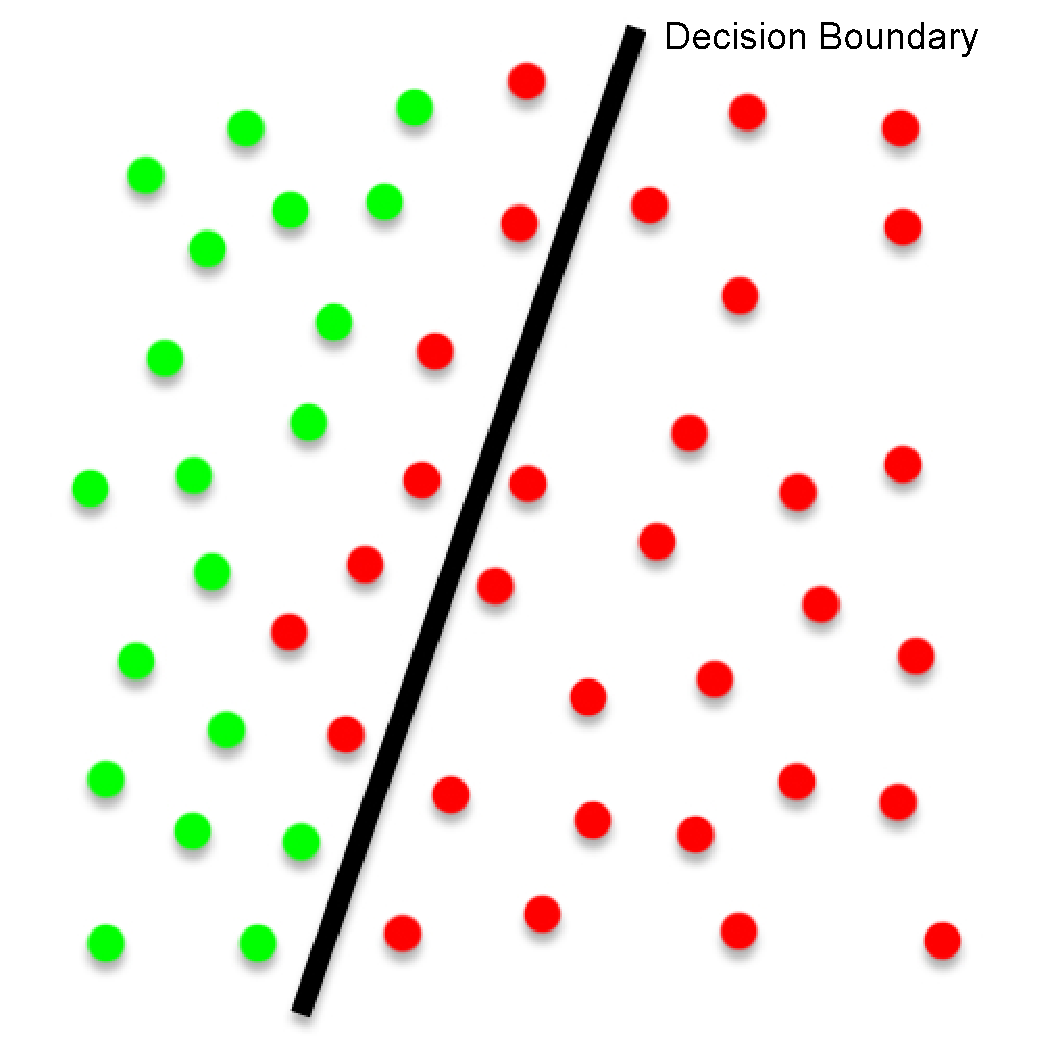
\includegraphics[width=0.5\linewidth]{Figures/Prune.pdf}
  \caption{Decision boundary created by classifier}
  \label{fig:Prune}
\end{figure}
As seen in \ref{fig:Prune}, these classifiers will create a decision boundary on the edges where green points are in the tour and red edges are not. Using repeated pruning, we can limit our data to edges that are part of the solution with few misclassified edges. After reducing the problem space, We can then execute an approximation algorithm on this smaller dataset in turn providing close to an approximate solution in significantly less time.


%%%%%%%%
\chapter{Project Workplan}
\begin{figure}[h]
    \centering
  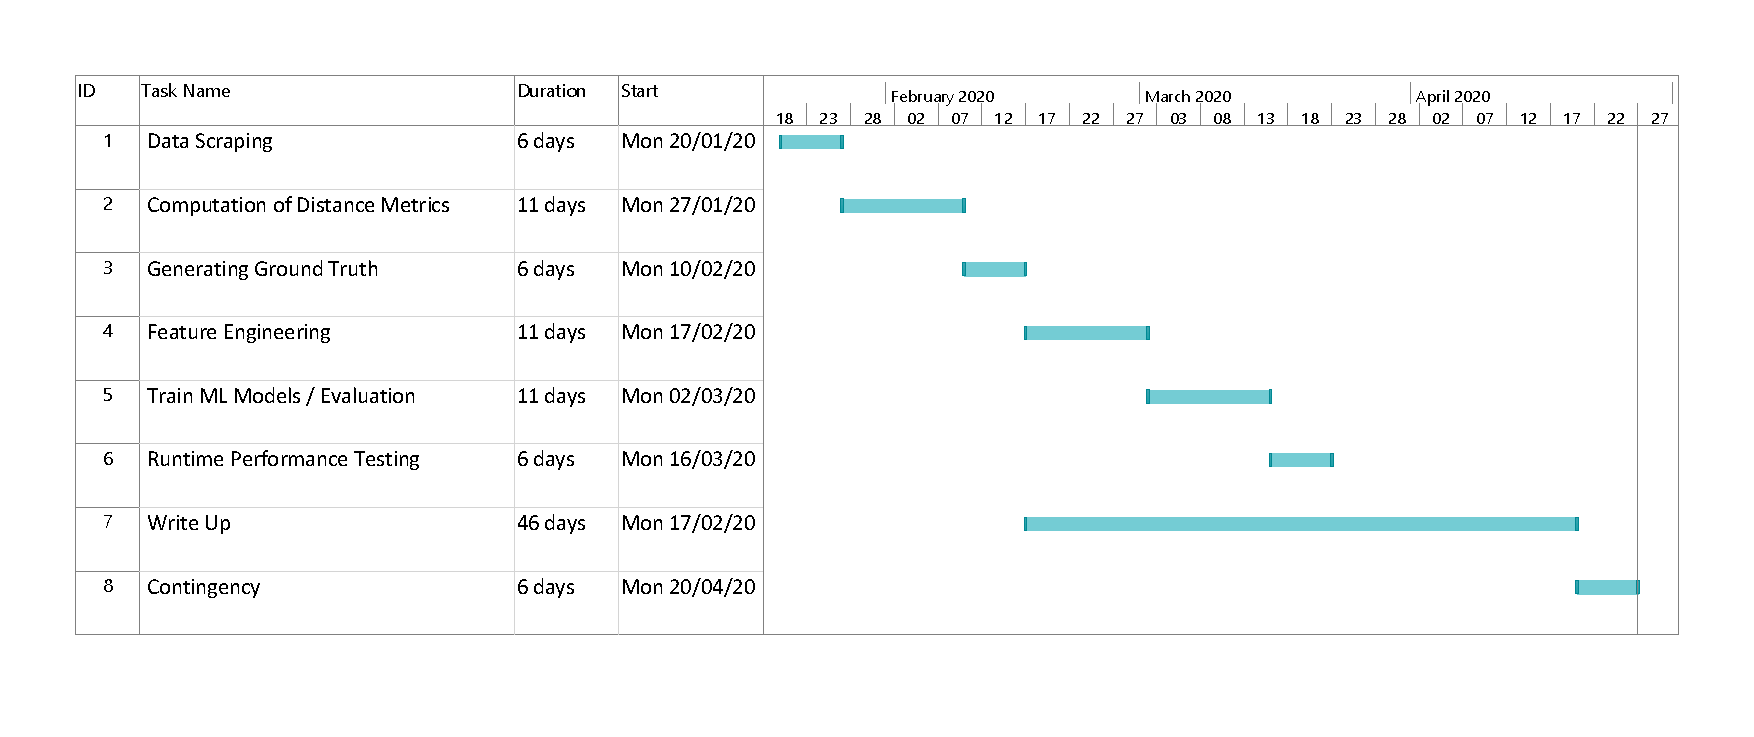
\includegraphics[width=1\linewidth]{Figures/GanttChart.pdf}
  \caption{Project Workplan}
  \label{fig:Workplan}
\end{figure}

\begin{itemize}
    \item \textbf{Data Scraping: }
    
    Writing the script to collect the data.
    \item \textbf{Data Cleaning/Pre-processing: }
    
    Cleaning the data and reformatting it into an edge list rather than a list of coordinates.
    \item \textbf{Generating Ground Truth: }
    
    Finding a close to optimal solution through other methods to generate the \textit{target} column in the data.
    \item \textbf{Characterizing Data: }
    
    Finding features that will capture details in the edges to aid in the classification process.
    \item \textbf{Train Machine Learning Models/Evaluation and Testing: }
    
    Training, paramaterizing, evaluating and testing the machine learning models.
    \item \textbf{Write Up: }
    
    Experimental write up.
    \item \textbf{Contingency: }
    
    I've allowed roughly one week for contingency for problems that will arise while carrying out this project. I believe this is an adequate amount of time tackle the upcoming problems.
\end{itemize}

%%%%%%%%
\chapter{Summary and Conclusions}
Combinatorial optimization is an NP-Hard problem that has applications in today’s world. In this paper we tackled the travelling salesman problem, one of the classical combinatorial optimization problems. Explored the state-of-the art and many methods of tackling the TSP from Exact algorithms to complex Deep Learning frameworks. We proposed a machine learning classification framework to learn the edges that are in the travelling salesman problem in order to prune edges that aren’t in the TSP. This enables us to run approximation algorithms on a considerably smaller edge list which will reduce computation time. 

There is a concern about the accuracy of the solution as we’ve opted to use Euclidean Distance measure between the pubs rather than path given by roads/ferries that could be provided by the Google Maps API, however we have a limited amount of API calls and this limits us to the method we have proposed.


%%%%%%%%%%%%%%%%%%%%%%
%%%% Latex help.
%\chapter{Latex Pointers}

This chapter contains some examples on the usage of latex. Do not include in your final report.

\section{Figures}
From time to time, it's necessary to add pictures to your documents. Using LaTeX all pictures will be indexed automatically and tagged with successive numbers when using the figure environment and the graphicx package. We can reference the figure below using its label like this: Fig. \ref{fig:test_plot}.
\begin{figure}[h]
    \centering
  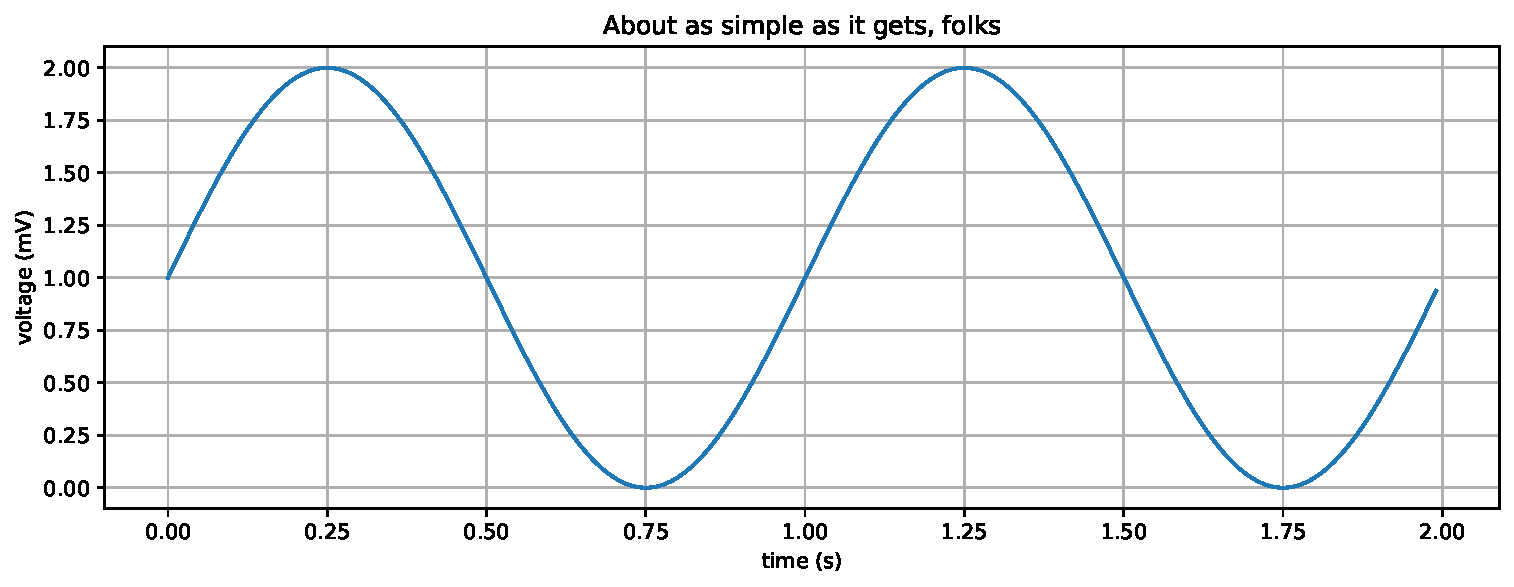
\includegraphics[width=0.8\linewidth]{test_plot.pdf}
  \caption{A sample graph}
  \label{fig:test_plot}
\end{figure}

Lots more information in this \href{https://www.latex-tutorial.com/tutorials/figures/}{tutorial}.


\section{Code Listing}
You can list code using the \emph{listings} package:

\begin{lstlisting}[language=Python,caption=Borg Pattern]
class Borg(object):
    __shared_state = {}

    def __init__(self):
        self.__dict__ = self.__shared_state
        self.state = 'Init'

    def __str__(self):
        return self.state
\end{lstlisting}

Lots more examples \href{https://www.overleaf.com/learn/latex/Code_listing}{here}.

\section{Math}
Here \ref{eq:limit} is an example of including an equation
\begin{equation}
\lim_{x\to\infty} f(x)
\label{eq:limit}
\end{equation}

More examples \href{https://www.latex-tutorial.com/tutorials/amsmath/}{here} and \href{https://www.overleaf.com/learn/latex/Mathematical_expressions}{here}.



\section{References}
Look up the bibtex references on google scholar or import from Mendeley or other reference managers. Add the bibtex snippet to the \emph{references.bib} file. Then cite the reference like this:

As explained in \cite{knuth2014art}, we also find that...

Lots more details \href{https://www.latex-tutorial.com/tutorials/bibtex/}{here}.


%%%%%%%%%%%%%%%%%%%%%%
%%% Acknowledgements
\chapter*{Acknowledgements}
I would like to thank University College Dublin’s school of Computer Science for their support and Dr. Deepak Ajwani for his guidance throughout this project.


%%%% ADD YOUR BIBLIOGRAPHY HERE
\printbibliography

%%%%
%%%% maybe code listing here?

%%%%
\end{document}
%\end{article}
